\documentclass[a4paper, 10pt, dvipdfmx]{jlreq}

\usepackage{amsmath,amsfonts,amssymb}
\usepackage{bm}
\usepackage{mathtools}
\usepackage{siunitx}
\usepackage[dvipdfmx]{graphicx}
\usepackage[dvipdfmx]{color}
\usepackage[dvipdfmx, colorlinks=true, allcolors=blue]{hyperref}
\usepackage{listings, jlisting}
\usepackage{tikz}
\usepackage{physics}
\usepackage{url}

\Urlmuskip=0mu plus 10mu
\allowdisplaybreaks[4]
\frenchspacing
\definecolor{OliveGreen}{rgb}{0.0,0.6,0.0}
\definecolor{Orenge}{rgb}{0.89,0.55,0}
\definecolor{SkyBlue}{rgb}{0.28, 0.28, 0.95}
\lstset{
  language={c++},
  basicstyle={\ttfamily},
  identifierstyle={\small},
  ndkeywordstyle={\small},
  frame=single,
  breaklines=true,
  numbers=left,
  xrightmargin=0zw,
  xleftmargin=3zw,
  numberstyle={\scriptsize},
  lineskip=-0.9ex,
  keywordstyle={\small\bfseries\color{SkyBlue}},  
  commentstyle={\color{OliveGreen}}, 
  stringstyle={\small\ttfamily\color{Orenge}}    
}

\begin{document}

\title{2012年度 大問4}
\author{hari64boli64 (hari64boli64@gmail.com)}
\date{\today}
\maketitle

\section{問題}

双対問題を用いた最適化

\section{解答}

\subsection*{(1),(2),(3)}

略

\subsection*{(4)}

(3)より、

\begin{align*}
  \text{Minimize} \quad   & s                                                           \\
  \text{subject to} \quad & 3x_1^2-4x_1x_2-2x_2^2+s \geq 0 \quad (\forall \bm{x} \in U)
\end{align*}

を解けばよい。

(2)より、

\begin{align*}
  3x_1^2-4x_1x_2-2x_2^2+s \geq & t_1(-2x_1^2-2x_1x_2-x_2^2+4)                         \\
  +                            & t_2(x_1^2-1) \quad (\forall \bm{x} \in \mathbb{R}^n)
\end{align*}

を満たす$t_1,t_2$が存在する範囲内で、$s$を最小化すればよい。

(1)より、

\begin{align*}
  \mqty(
  3+2t_1-t_2 & -2+t_1 &            \\
  -2+t_1     & -2+t_1 &            \\
             &        & s-4t_1+t_2
  ) \succeq 0
\end{align*}

の下で、$s$を最小化すればよい。

則ち、

\begin{align*}
  \mqty(
  3+2t_1-t_2 & -2+t_1 \\
  -2+t_1     & -2+t_1
  ) \succeq 0
\end{align*}

の下で、$4t_1-t_2$を最小化すればよい。


{\color{lightgray}

これは、固有値を求めた上で考えると、解の配置問題である。

尤も、直接解くのはかなり厳しい。

しかし、適当に考えると、$t_1=2,t_2=7$の時、固有値は共に0で、目的関数の値は1になる。
}

そして、$x_1=1,x_2=-1+\sqrt{3}$を代入すると、確かに元の最適化問題において、制約を満たした上で、これの目的関数も1になる。

以上より、$s=1$が最適解である。

{\color{lightgray}

なお、後半3行は計算機パワーを用いたチートであり、試験の上では、(3),(2),(1)を用いた変形さえ出来ていれば、十分ではないかと思われる。

}

{\color{red}

普通に小行列式に注目すると解ける。

}

\section{おまけ}

\lstinputlisting[caption=vis,label=code:vis,language=Python]{4.py}

\begin{figure}[htbp]
  \begin{center}
    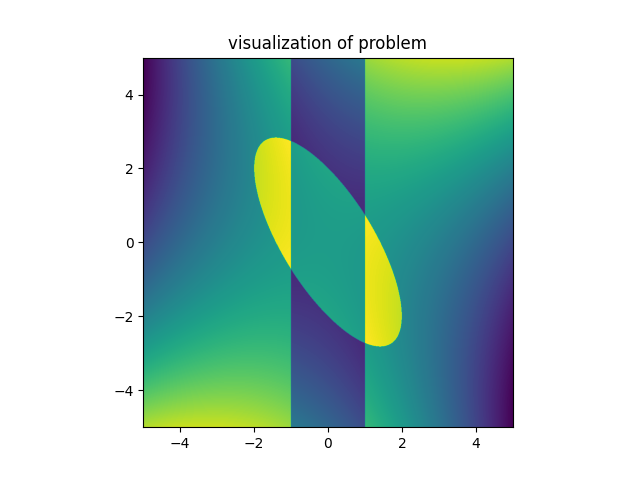
\includegraphics[height=80mm]{4_vis.png}
    \caption{イメージ図}
  \end{center}
\end{figure}

\begin{figure}[htbp]
  \begin{center}
    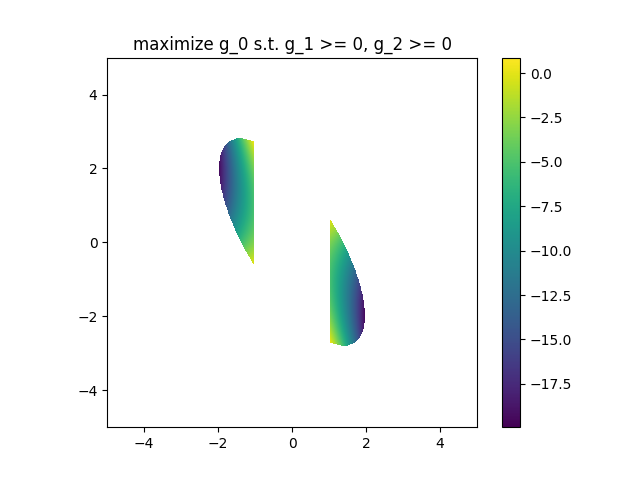
\includegraphics[height=80mm]{4_actual.png}
    \caption{総当たりによる実際の図}
    \label{img:label}
  \end{center}
\end{figure}

1個目の条件式は、とある楕円形内部の点であることを表す。

2個目の条件式は、$x_1 \leq -1$、または、$x_1 \geq 1$を表す。

目的関数は右上と左下の値が高い、双曲線のような形をしている。

そのことに対応した図であることが読みとれるかと思われる。

\end{document}
